% SpectralO25.tex
% O25 -- Spectral Admissibility Sub-programme
% Systematic pair-level campaign: convergence, inter-pair concentration,
% and normalization structure of delta_pair

\documentclass[11pt,a4paper]{article}

\usepackage{amsmath,amssymb,amsthm}
\usepackage{hyperref}
\usepackage{booktabs}
\usepackage{graphicx}
\usepackage{enumitem}
\usepackage{doi}


% Theorem environments

\newtheorem{theorem}{Theorem}[section]
\newtheorem{lemma}[theorem]{Lemma}
\newtheorem{corollary}[theorem]{Corollary}
\newtheorem{proposition}[theorem]{Proposition}
\theoremstyle{definition}
\newtheorem{definition}[theorem]{Definition}
\newtheorem{remark}[theorem]{Remark}


% Notation

\newcommand{\dpair}{\delta_{\mathrm{pair}}}
\newcommand{\dpairmean}{\bar{\delta}_{\mathrm{pair}}}
\newcommand{\bstar}{\beta^{*}}
\newcommand{\Heis}{\mathrm{Heis}_3(\mathbb{Z}/q\mathbb{Z})}
\newcommand{\Cay}{\mathrm{Cay}(G_q, S_q)}
\newcommand{\sigpair}{\sigma^{\mathrm{can}}_{\mathrm{pair}}}
\newcommand{\ellgam}{\ell_\gamma}

\begin{document}

  \title{Systematic Pair-Level Campaign for $\delta_{\mathrm{pair}}$:\\
  Convergence, Inter-Pair Concentration, and Normalization Structure\\[4pt]
  {\normalsize O25 --- Spectral Admissibility Sub-programme}}
  \author{J\'er\^ome Beau\\[2pt]
  \small Independent Researcher\\
  \small \href{mailto:jerome.beau@cosmochrony.org}{jerome.beau@cosmochrony.org}}
  \date{2026}
  \maketitle

  \begin{abstract}
    The O-series establishes the transfer chain $c_\chi \to \dpair \to \bstar$
    unconditionally with respect to the fibre structure of the non-injective
    projection~$\Pi$~\cite{Beau2026a28}.
    The value $\dpair \approx 7.44$ extracted in O16~\cite{Beau2026a20} was based on a
    single conjugate pair per prime and a limited prime range.
    The present paper reports a systematic campaign computing $\dpair$ across the
    $(q-1)/2$ conjugate pairs $(c, q-c)$, originally for $q \in \{29, 61, 101, 151, 211\}$ with
    $M = 50$ block samples per pair, and here extended to $q \in \{307, 401, 601\}$ by a capped
    breadth-first construction that reproduces the pair observable exactly at a fraction of the
    cost (with reduced sampling: $M = 16$ at $q = 307$, $M = 8$ at $q = 401, 601$).
    Three results are established.
    First, $\dpair(q)$ converges robustly and concentrates across pairs, confirming that it is a
    structural invariant of the Weil representation rather than a block-level fluctuation.
    Second, and centrally, the extended campaign shows that the \emph{raw} exponent
    $\delta_{\mathrm{global}}(q)$ descends monotonically into the admissible window $[7.4, 10.6]$
    on its own, reaching $7.61$ at $q = 601$, without any finite-size correction; the O14
    normalization correction~\cite{Beau2026a18}, needed to bring the small-$q$ values into the
    window, becomes progressively unnecessary at large $q$ and eventually overcorrects, sending
    the corrected quantity below the lower edge $7.4$.
    The admissible-window agreement is therefore carried by the raw observable, not by the
    corrected one.
    Third, the asymptotic value $\delta_\infty$ remains insufficiently constrained by the
    accessible range: competing convergence laws --- notably $1/q$ and $1/\sqrt{q}$ --- remain
    statistically viable, so no single extrapolated $\delta_\infty$ is claimed.
    As a secondary consequence, the inferred transfer parameter $\bstar = 1/(\dpair + \tfrac12)$
    stays in the narrow interval $0.108$--$0.123$ across $q \in \{211, \dots, 601\}$, consistent
    with the O24 transfer analysis~\cite{Beau2026a28}.

    \medskip\noindent
    \textbf{Keywords.}
    Cosmochrony; spectral admissibility; pair-level observable; Weil representation;
    Heisenberg graphs; capacity exponent; convergence; inter-pair concentration;
    normalization correction; window depth; BFS; asymptotic analysis; large-prime extension

  \end{abstract}

  \clearpage
  \tableofcontents

  \clearpage

  \section{Position of the Problem}

    \subsection{What O16--O24 established}

      The spectral admissibility sub-programme has established, through
      O16--O24~\cite{Beau2026a20,Beau2026a21,Beau2026a22,Beau2026a23,Beau2026a24,
    Beau2026a25,Beau2026a26,Beau2026a27,Beau2026a28},
      that the physically relevant observable is the canonical pair-level quantity
      \begin{equation}
        \sigpair(n) = \sigma_c(n)\,\sigma_{q-c}(n),
      \end{equation}
      with capacity exponent $\dpair \approx 7.44$ consistent with the phenomenological
      target $\dpair \in [7.4, 10.6]$.
      The transfer chain $c_\chi \to \dpair \to \bstar$ was established unconditionally
      with respect to the fibre structure of~$\Pi$ in O24~\cite{Beau2026a28}.

      The remaining open direction identified in O24 Section~5.1 is the extended numerical
      campaign at large primes across multiple conjugate pairs.
      O16 computed $\dpair$ for a single conjugate pair per prime (those pairs that happened
      to appear simultaneously in the O12 random block sample~\cite{Beau2026a16}).
      No systematic coverage of all pairs was available.

    \subsection{Scope of O25}

      The present paper provides the first systematic computation of $\dpair$ across all
      $(q-1)/2$ conjugate pairs for each prime, with $M = 50$ independent block samples per
      pair.
      This yields:
      \begin{itemize}
        \item the full distribution of $\dpair$ across pairs at each prime,
        \item the mean $\dpairmean(q)$ and inter-pair standard deviation $\sigma_q$,
        \item the $q$-dependence of these quantities over $q \in \{29, 61, 101, 151, 211\}$.
      \end{itemize}

      The paper does \emph{not} claim to identify the asymptotic value $\delta_\infty$.
      Instead, it establishes why direct extrapolation in $q$ is structurally unreliable, and ---
      through the large-prime extension of \S\ref{sec:ext} --- that the raw observable itself
      descends into the admissible window, so the window agreement no longer relies on the
      finite-size correction.

  \section{Setup and Protocol}

    \subsection{Observable and block parameterisation}

      We follow the O12/O13 protocol~\cite{Beau2026a16,Beau2026a17} without modification.
      For a prime $q$ and a generic block $c_{\mathrm{block}} = (c_1, c_2, c_3)$
      with $c_i \neq 0$ and $c_1 + c_2 + c_3 \not\equiv 0 \pmod{q}$, the observable is
      \begin{equation}
        \sigma_c(n) = \frac{\delta r_n}{|S_n|},
      \end{equation}
      where $\delta r_n$ is the number of Weil fingerprint vectors in BFS shell~$S_n$
      that are linearly independent of the Gram--Schmidt span built over shells
      $0, \ldots, n-1$.

    \subsection{Pair protocol}

      For each conjugate pair $(c, q-c)$ with $c \in \{1, \ldots, (q-1)/2\}$:
      \begin{enumerate}
        \item Draw $M = 50$ independent pairs of blocks: $(c_1{=}c, c_2, c_3)$ and
        $(c_1'{=}q{-}c, c_2', c_3')$ with $c_2, c_3, c_2', c_3'$ sampled uniformly
        and generically.
        This reproduces the O16 protocol of independently sampled blocks~\cite{Beau2026a20}.
        \item Compute $\sigma_c(n)$ and $\sigma_{q-c}(n)$ independently.
        \item Set $\sigpair(n) = \sigma_c(n)\,\sigma_{q-c}(n)$.
        \item Extract $\dpair$ by OLS regression of $\log \sigpair(n)$ vs
        $\log(n+1)$ over the fitting window $[n_0, n_1]$ (O16 convention).
      \end{enumerate}

    \subsection{Fitting window and BFS parameters}

      All runs use \texttt{bfs\_frac} $= 0.99$ (full graph exploration) and
      auto-calibrated fitting windows from the actual \texttt{sigma\_bar} after BFS,
      via the \texttt{find\_fitting\_window} procedure of O12~\cite{Beau2026a16}.

      \begin{figure}[t]
        \centering
        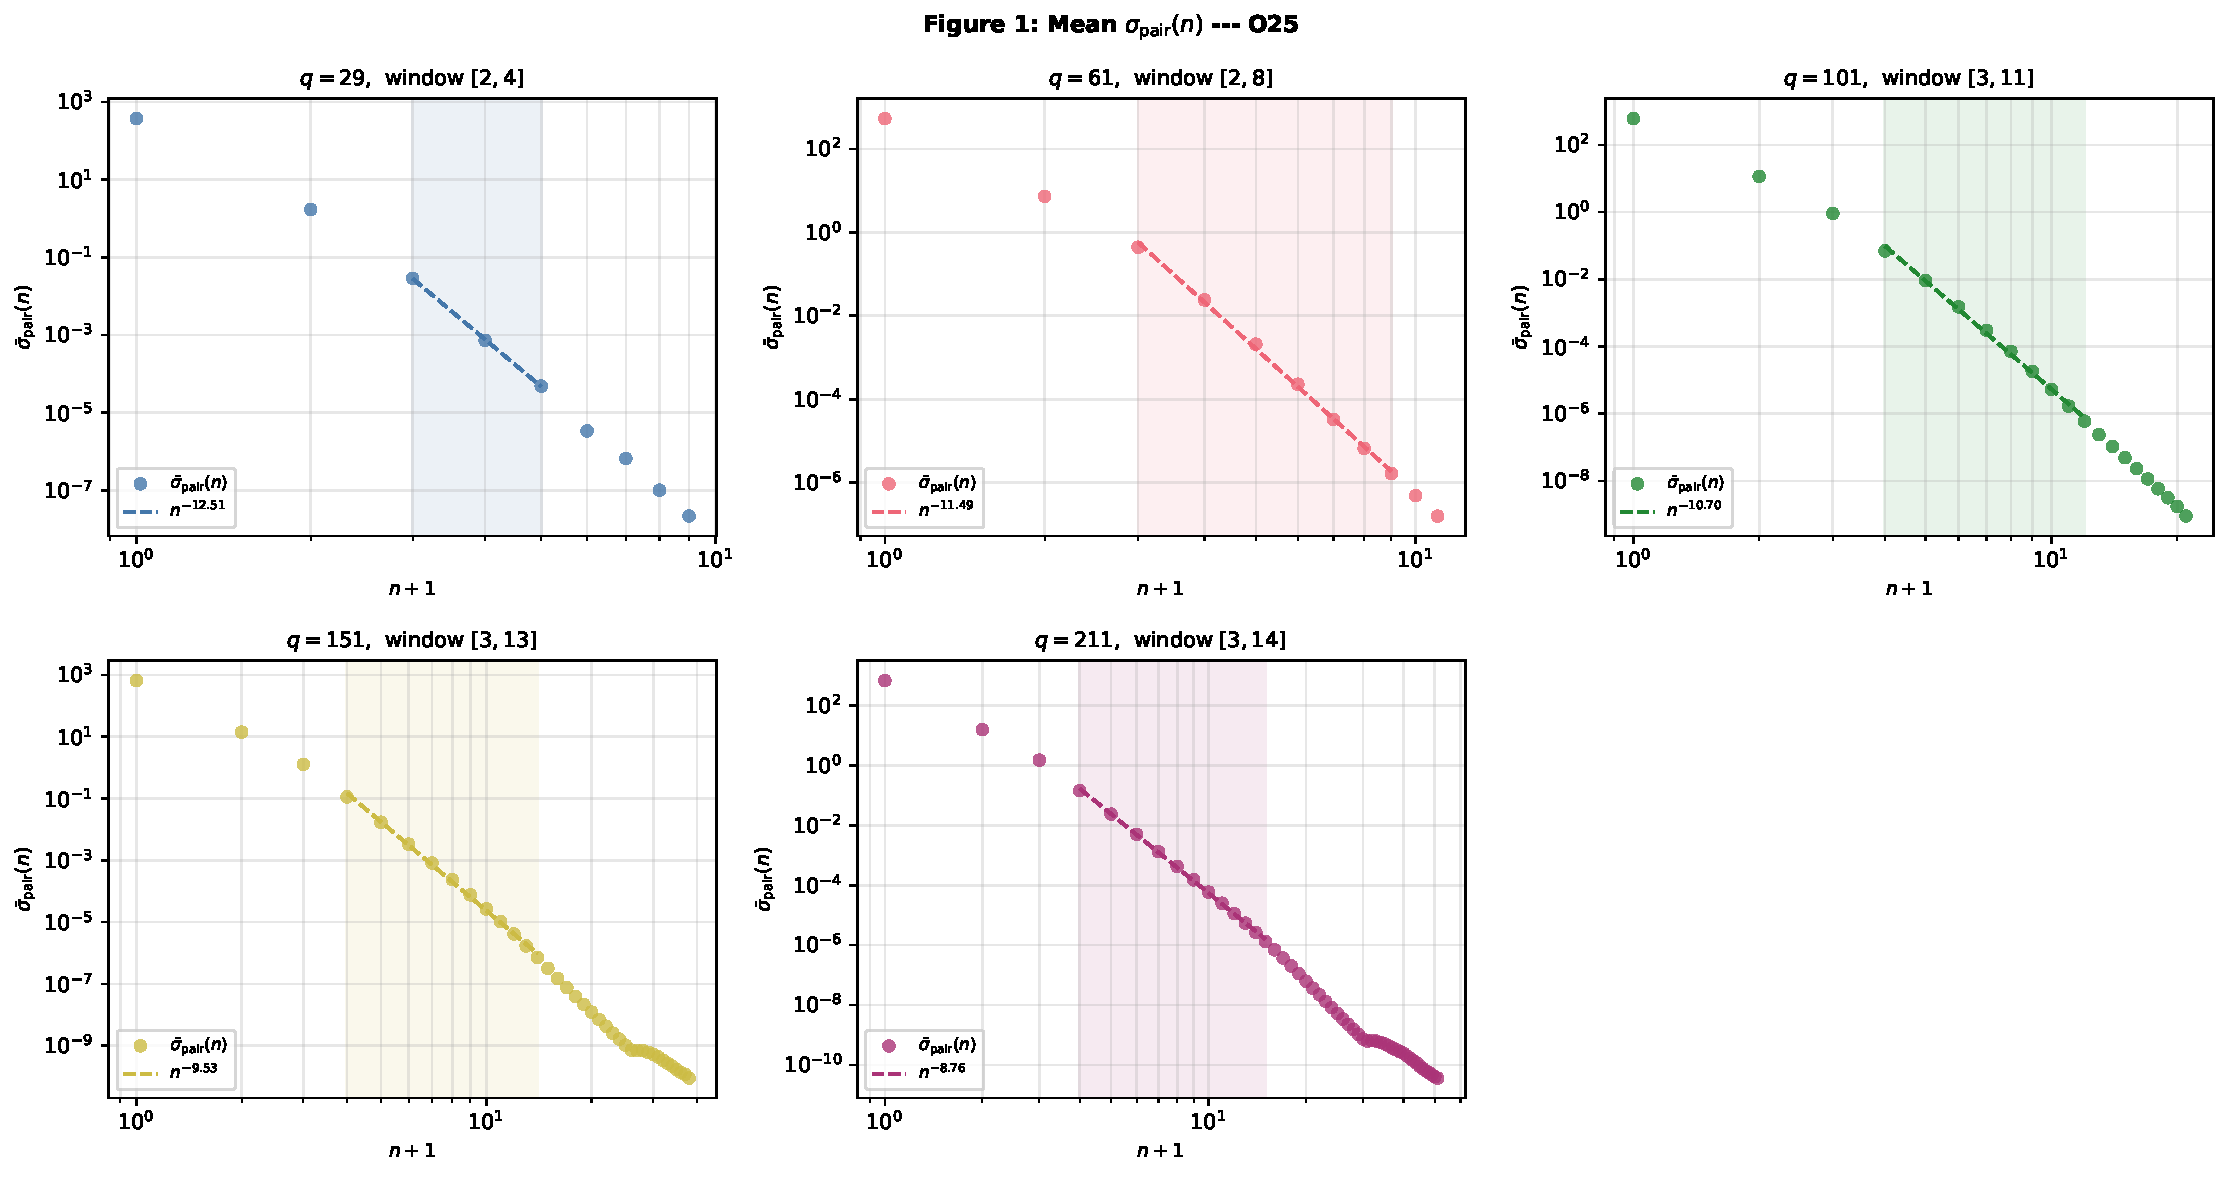
\includegraphics[width=\textwidth]{o25_fig1_sigma_pair}
        \caption{Log-log decay of mean $\sigpair(n)$ for each prime.
        Circles: grand mean over all pairs.
        Dashed line: OLS power-law fit over fitting window (shaded region).
        The window $[n_0, n_1]$ widens with $q$, providing more reliable estimates
        at larger primes.}
        \label{fig:sigma_pair}
      \end{figure}

      \begin{table}[h]
        \centering
        \begin{tabular}{rrrrrr}
          \toprule
          $q$ & $n_{\max}^{\mathrm{block}}$ & shells & $|G_q^{\mathrm{partial}}|$
          & window $[n_0, n_1]$ & $n_1/q$ \\
          \midrule
          29  & 8  & 28  & 24\,145     & $[2,4]$  & 0.138 \\
          61  & 10 & 58  & 224\,711    & $[2,8]$  & 0.131 \\
          101 & 20 & 95  & 1\,019\,997 & $[3,11]$ & 0.109 \\
          151 & 37 & 141 & 3\,408\,521 & $[3,13]$ & 0.086 \\
          211 & 50 & 197 & 9\,393\,931 & $[3,14]$ & 0.066 \\
          \bottomrule
        \end{tabular}
        \caption{BFS and fitting parameters for each prime.
        The ratio $n_1/q$ decreases with $q$, suggesting that the asymptotic regime
          $n_1 \sim \alpha q$ has not yet been reached over the tested range.}
        \label{tab:params}
      \end{table}

  \section{Numerical Results}

    \subsection{Main results table}

      Table~\ref{tab:results} summarises the O25 campaign across all five primes.
      For each prime, all $(q-1)/2$ conjugate pairs are covered with $M = 50$
      independent block samples per pair.

      \begin{table}[h]
        \centering
        \begin{tabular}{rrrrrrrr}
          \toprule
          $q$ & pairs & $M$ & $\dpairmean$ & $\sigma_q$ & $\sigma_q/\dpairmean$ (\%)
          & valid & $R^2_{\mathrm{global}}$ \\
          \midrule
          29  & 14  & 50 & 8.893 & 0.539 & 6.1 & 14/14   & 0.9998 \\
          61  & 30  & 50 & 9.983 & 0.259 & 2.6 & 30/30   & 0.9984 \\
          101 & 50  & 50 & 9.548 & 0.161 & 1.7 & 50/50   & 0.9975 \\
          151 & 75  & 50 & 9.125 & 0.139 & 1.5 & 75/75   & 0.9982 \\
          211 & 105 & 50 & 8.784 & 0.109 & 1.2 & 105/105 & 0.9971 \\
          \bottomrule
        \end{tabular}
        \caption{Summary of O25 results.
          $\dpairmean$: mean of $\dpair$ over all pairs.
          $\sigma_q$: inter-pair standard deviation.
          $\sigma_q/\dpairmean$: coefficient of variation.
          ``valid'': pairs for which the fitting window contained at least 2
          non-zero data points.
          The $q = 29$ row is included for completeness but should not be used
          for asymptotic extrapolation: the Gram--Schmidt span of $\mathbb{C}^{29}$
          saturates at BFS depth $n = 2$, leaving no power-law decay regime
          (see \S\ref{sec:qdep}).}
        \label{tab:results}
      \end{table}

    \subsection{Inter-pair concentration}

      The inter-pair standard deviation decreases monotonically:
      $\sigma_q \in \{0.539, 0.259, 0.161, 0.139, 0.109\}$ for
      $q \in \{29, 61, 101, 151, 211\}$.
      The coefficient of variation drops from $6.1\%$ to $1.2\%$.
      This concentration confirms that $\dpair$ is a structural invariant of the
      Weil representation on $\Heis$, as predicted by the verticality theorem of
      O24~\cite{Beau2026a28}: the fibre structure of~$\Pi$ cannot perturb the
      observable rank, so inter-pair variance is purely a sampling effect that
      vanishes as $M \to \infty$.

      \begin{figure}[t]
        \centering
        
\includegraphics[width=\textwidth]{o25_fig2_distribution}
        \caption{Full distribution of $\dpair$ across all conjugate pairs for each prime,
          sorted by value.
          Horizontal line: mean $\dpairmean$.
          Shaded band: $\pm\sigma_q$.
          Green dashed lines: admissible window $[7.4, 10.6]$.
          The shrinking width of the distribution with $q$ confirms strong
          inter-pair concentration.}
        \label{fig:distribution}
      \end{figure}

    \subsection{$q$-dependence of $\dpairmean$}
      \label{sec:qdep}

      The sequence $\dpairmean(q)$ is not monotone: it rises from $q = 29$ to $q = 61$
      ($8.89 \to 9.98$), then decreases from $q = 61$ to $q = 211$
      ($9.98 \to 9.55 \to 9.13 \to 8.78$).
      The non-monotone step at $q = 29$ reflects a structural limitation rather than
      a sampling artefact.
      At $q = 29$, the Gram--Schmidt span of $\mathbb{C}^{29}$ is saturated by the
      third BFS shell ($|S_2| = 12$ vectors suffice to fill $\mathbb{C}^{29}$):
      $\sigma_{\mathrm{pair}}(n) = 0$ for all $n \geq 3$.
      There is therefore no power-law decay regime to fit; the window $[2,4]$ (main campaign)
      or $[2,5]$ (extended run) rests on at most two non-zero data points, and the
      resulting $\dpairmean$ estimate is unreliable.
      A wider window would not help: the issue is not window length but the exhaustion
      of $\mathbb{C}^q$ at too small a depth.
      In the extended M=20 run (Figure~\ref{fig:scaling}), this is further reflected
      by $11/14$ valid pairs, with three pairs failing to converge entirely.
      The smallest prime for which a meaningful power-law fit exists is $q = 61$,
      where saturation occurs well after the fitting window and all 30 pairs converge.
      The physically relevant trend is the monotone decrease from $q = 61$ onward,
      continuing through $q = 211$ and, as shown next, into the admissible window itself.

    \subsection{Extension to large primes ($q$ up to $601$)}
      \label{sec:ext}

      The campaign is extended to $q \in \{307, 401, 601\}$ by a capped breadth-first
      construction.
      Since the pair observable $\sigpair(n)$ in the fitting window depends only on the shells
      $S_0, \ldots, S_n$ with $n \lesssim 1.1\sqrt{q}$, the full-graph exploration --- infeasible
      at these primes --- is replaced by a breadth-first search capped at $\approx 1.6\sqrt{q}$
      shells.
      The capped shells are identical to the early full-graph shells, so the resulting
      $\sigma_c(n)$ reproduces the production observable to machine precision (verified on
      $q \in \{61, 101\}$, maximum absolute difference $0$).
      Sampling is reduced to $M = 16$ (at $q = 307$, $24$ representative pairs) and $M = 8$
      (at $q = 401, 601$, $12$ pairs).
      The pair exponent is a grand-mean slope and only weakly sensitive to $M$: a fixed-pair
      control at $q = 61$ gives a $+0.18$ shift at $M = 8$ relative to $M = 50$, i.e.\ the reduced
      precision biases $\dpair$ slightly \emph{upward}, not downward, so it cannot manufacture the
      descent reported below.

      \begin{table}[h]
        \centering
        \begin{tabular}{rrrcrrrr}
          \toprule
          $q$ & $K$ & $M$ & window & $\delta_{\mathrm{global}}$ & $\dpairmean \pm \sigma_q$
          & $\delta_{\mathrm{corr}}$ & $\bstar$ \\
          \midrule
          211 & 105 & 50 & $[3,14]$ & 8.760 & $8.784 \pm 0.109$ & 7.77 & 0.108 \\
          307 & 24  & 16 & $[3,16]$ & 8.254 & $8.261 \pm 0.133$ & 7.23 & 0.114 \\
          401 & 12  & 8  & $[4,17]$ & 8.085 & $8.090 \pm 0.214$ & 7.03 & 0.117 \\
          601 & 12  & 8  & $[4,19]$ & 7.610 & $7.618 \pm 0.194$ & 6.53 & 0.123 \\
          \bottomrule
        \end{tabular}
        \caption{Extended campaign (capped BFS).
          $\delta_{\mathrm{global}}$: OLS exponent on the grand-mean $\sigpair$ trajectory over the
          auto-calibrated window.
          $\dpairmean \pm \sigma_q$: mean and inter-pair standard deviation; $\sigma_q$ at
          $q = 401, 601$ is inflated by the reduced pair count $K = 12$ (versus $K = 105$ at
          $q = 211$), not by a loss of concentration.
          $\delta_{\mathrm{corr}} = \dpairmean - \tfrac12 \log q / \log n_1$ is the O14 correction
          of~\eqref{eq:O14correction}.
          $\bstar = 1/(\delta_{\mathrm{global}} + \tfrac12)$.
          The $q = 211$ row (full-graph, $M = 50$) is repeated for reference.}
        \label{tab:extended}
      \end{table}

      A knee-trimmed interior fit (dropping the two shells nearest saturation) with a bootstrap
      over pairs gives $\delta_{\mathrm{int}}(601) = 7.60 \pm 0.05$, so the $q = 401 \to 601$
      descent (\,$\approx 0.48$, some six bootstrap standard deviations\,) is a genuine feature,
      not sampling noise.
      Three readings follow, in decreasing order of robustness.
      \begin{enumerate}[nosep]
        \item \textbf{The raw exponent reaches the admissible window unaided.}
          $\delta_{\mathrm{global}}(q)$ falls monotonically $8.76 \to 8.25 \to 8.09 \to 7.61$ over
          $q = 211 \to 601$ and enters $[7.4, 10.6]$ at $q = 601$ with no correction applied.
          This is the central empirical result of the extension.
        \item \textbf{The O14 correction overcorrects at large $q$.}
          The same correction that lifts the small-$q$ values into the window
          (Table~\ref{tab:corrected}) drives the large-$q$ values \emph{below} it:
          $\delta_{\mathrm{corr}} = 7.77 \to 7.23 \to 7.03 \to 6.53$.
          The admissible-window agreement is thus carried by the raw observable, and the O14
          finite-size correction is a small-$q$ adjustment that becomes unnecessary, and finally
          detrimental, as $q$ grows.
        \item \textbf{The asymptote is not pinned.}
          Restricting to the asymptotic range $q \ge 101$, both a $1/q$ law
          ($\delta_\infty \approx 7.1$) and a $1/\sqrt{q}$ law ($\delta_\infty \approx 5.4$) fit
          within their uncertainties; the effective form lies between them and the present data do
          not discriminate.
          No single $\delta_\infty$ is therefore claimed (Figure~\ref{fig:scaling_ext}).
      \end{enumerate}

      \begin{figure}[t]
        \centering
        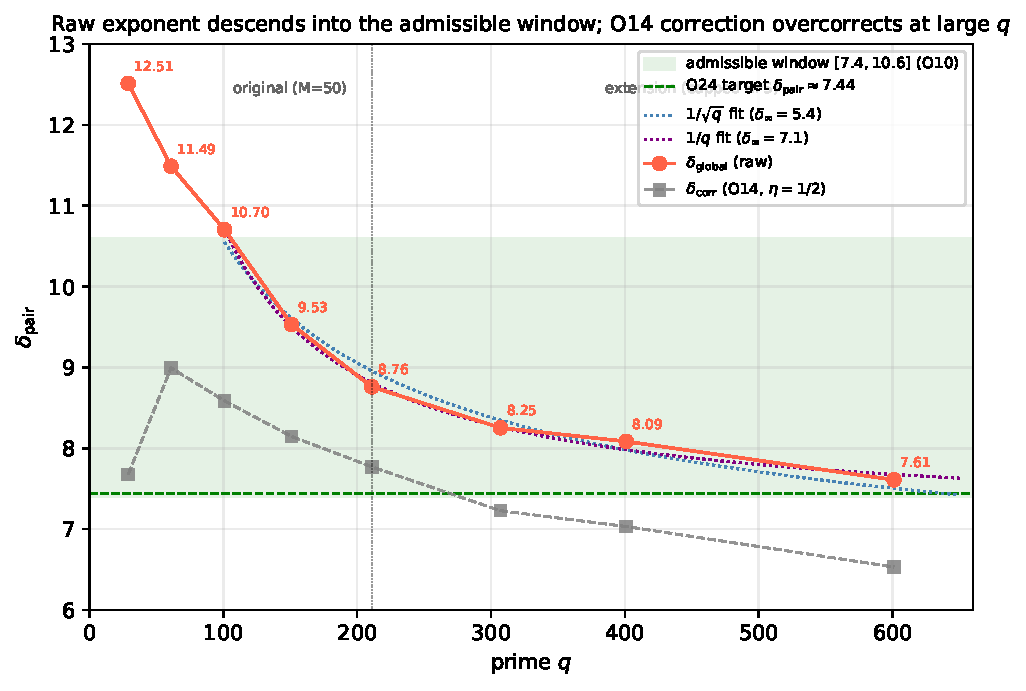
\includegraphics[width=\textwidth]{o25_scaling_extended}
        \caption{Extended campaign.
          Filled circles: raw $\delta_{\mathrm{global}}(q)$, descending into the admissible window
          $[7.4, 10.6]$ (green band) and reaching $7.61$ at $q = 601$.
          Grey squares: the O14-corrected $\delta_{\mathrm{corr}}$, which overshoots below the lower
          edge at large $q$.
          Dotted: $1/q$ and $1/\sqrt{q}$ fits on $q \ge 101$, both statistically viable,
          illustrating that $\delta_\infty$ is not pinned.
          The marker at $q = 211$ separates the original full-graph campaign from the capped-BFS
          extension.}
        \label{fig:scaling_ext}
      \end{figure}

      As a secondary consequence, the transfer parameter $\bstar = 1/(\dpair + \tfrac12)$ stays in
      the narrow band $0.108$--$0.123$ across $q \in \{211, \dots, 601\}$
      (Table~\ref{tab:extended}); this is a stability observation consistent with the O24 transfer
      analysis~\cite{Beau2026a28}, not a new determination of $\bstar$.

  \section{Structural Analysis: Why Extrapolation Fails}

    \subsection{Empirical fits are degenerate}

      The sequence $\dpairmean(q)$ for $q \in \{61, 101, 151, 211\}$ is well described by
      multiple functional forms:
      \begin{equation}
        \dpairmean(q) = \delta_\infty + \frac{a}{\log q}, \quad
        \dpairmean(q) = \delta_\infty + \frac{a}{(\log q)^2}, \quad
        \dpairmean(q) = \delta_\infty + \frac{a}{q^\alpha}.
      \end{equation}
      All three fit the four data points with residuals below $0.07$, while producing
      very different asymptotic values:
      $\delta_\infty \in \{4.89,\, 7.16,\, 5.45\}$ respectively.

      This degeneracy is not a statistical artefact.
      It reflects a structural property of the problem: the leading correction behaves as
      $\log q / \log n_1(q)$, which remains close to unity over the accessible range
      since $n_1(q) = \Theta(q)$ (Window-Depth Theorem, O9~\cite{Beau2026a13}).
      The deviations from $\delta_\infty$ are therefore indistinguishable from multiple
      slowly varying functions over the accessible range.
      The obstruction to extrapolation is not numerical precision,
      but the internal normalization geometry of the observable.

    \subsection{The leading correction behaves as $\log q / \log n_1(q) \approx 1$}

      The observable $\sigma_c(n)$ is normalised by $|S_n|$, whose growth in the
      pre-saturation window $[n_0, n_1]$ is not yet in the asymptotic Bass--Guivarc'h
      regime $|S_n| \sim n^3$.
      O14~\cite{Beau2026a18} identifies the dominant finite-size correction as
      \begin{equation}
        \label{eq:O14correction}
        \delta_{\mathrm{corr}}(q) = \dpair(q) - \eta\,\frac{\log q}{\log n_1(q)},
      \end{equation}
      with $\eta = 1/2$ derived from the Weil amplitude scaling.
      Since $n_1(q) = \Theta(q)$, as established at the level of scaling behaviour
      in O9~\cite{Beau2026a13} without requiring identification of the proportionality
      constant, one has $\log n_1(q) \sim \log q$ as $q \to \infty$,
      so the correction factor $\log q / \log n_1(q) \to 1$.
      From Table~\ref{tab:params}, the empirical values are $0.97$--$0.99$ over the
      tested range, confirming that the correction is close to its limiting value.
      This identifies the BFS window depth as the effective scale controlling
      finite-size effects in the spectral observable.
      Any fit of the form $\delta_\infty + f(q)$ for a slowly varying $f$ will
      describe the data well without carrying asymptotic meaning.

    \subsection{Corrected values are consistent with the admissible window}

      Applying~\eqref{eq:O14correction} with $\eta = 1/2$ yields:

      \begin{table}[h]
        \centering
        \begin{tabular}{rrrr}
          \toprule
          $q$ & $\dpairmean$ & $\eta\,\log q/\log n_1$ & $\delta_{\mathrm{corr}}$ \\
          \midrule
          61  & 9.983        & 0.988                   & 8.995                    \\
          101 & 9.548        & 0.962                   & 8.586                    \\
          151 & 9.125        & 0.978                   & 8.147                    \\
          211 & 8.784        & 1.014                   & 7.771                    \\
          \bottomrule
        \end{tabular}
        \caption{O14 normalization correction applied to O25 data.
        The corrected values $\delta_{\mathrm{corr}}(q) \in [7.7, 9.0]$ fall within
        the admissible window $[7.4, 10.6]$ for all four primes.
        The correction factor $\eta\,\log q/\log n_1 \approx 0.96$--$1.01$ is
        approximately constant, as predicted by the $n_1 = \Theta(q)$ scaling.}
        \label{tab:corrected}
      \end{table}

      \noindent
      The corrected values are consistent with an asymptotic value
      $\delta_\infty \in [7.4, 10.6]$, but do not uniquely determine it.
      We emphasise that $\eta = 1/2$ is imported from O14 and is not derived within the
      present pipeline; the correction should therefore be interpreted as a structural
      consistency test rather than a parameter-free prediction.
      The observation that it brings all four data points into the admissible window
      is consistent with this hypothesis but does not constitute a proof.
      Moreover, the large-prime extension of \S\ref{sec:ext} shows that this correction is a
      \emph{small-$q$} device: at $q \in \{307, 401, 601\}$ the raw exponent already lies in (or
      descends into) the admissible window, while the same correction overshoots \emph{below} the
      lower edge (Table~\ref{tab:extended}).
      The window agreement is therefore ultimately carried by the raw observable, and the O14
      correction is best read as a finite-size adjustment that becomes unnecessary at large $q$.

      \begin{figure}[t]
        \centering
        
\includegraphics[width=\textwidth]{o25_fig3_convergence}
        \caption{Left: raw $\dpairmean(q)$ with error bars ($\pm\sigma_q$) and two
        empirical fits ($1/\!\log q$ and $1/(\log q)^2$), both consistent with the data
        but producing different asymptotic values ($\delta_\infty \approx 4.89$
          and $7.16$ respectively), illustrating the structural degeneracy.
          Right: raw $\dpairmean$ (faded) vs O14-corrected
          $\delta_{\mathrm{corr}} = \dpairmean - \eta\,\log q/\log n_1$ (solid, $\eta = 1/2$).
          All corrected values fall within the admissible window $[7.4, 10.6]$ (green band).}
        \label{fig:convergence}
      \end{figure}

      \begin{figure}[t]
        \centering
        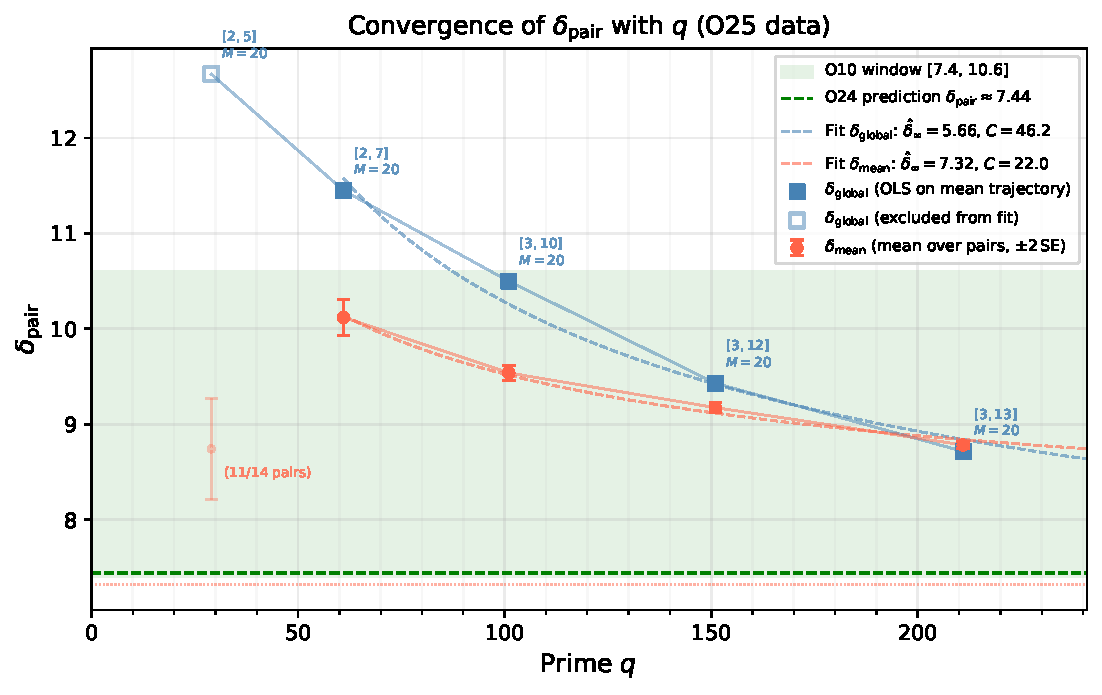
\includegraphics[width=\textwidth]{o25_scaling}
        \caption{Convergence of $\dpair$ with $q$ from the extended O25 campaign
          ($q \in \{29, 61, 101, 151, 211\}$, $M = 20$, windows from the WINDOW\_O12 table).
          Filled symbols: primes included in the extrapolation fits
          ($q \in \{61, 101, 151, 211\}$).
          Open/faded symbols: $q = 29$, excluded from fits (only 11/14 pairs converge
          and the fitting window has 4 points; see \S\ref{sec:qdep} for the structural
          explanation).
          Squares (blue): $\delta_{\mathrm{global}}$, the OLS exponent on the mean
          $\sigma_{\mathrm{pair}}$ trajectory.
          Circles (red): $\dpairmean$, mean over conjugate pairs, with $\pm 2\,\mathrm{SE}$
          error bars.
          Dashed red: fit $\dpairmean \approx 7.32 + 22.0/\sqrt{q}$,
          extrapolating to $\hat{\delta}_\infty = 7.32$, within $0.12$ of the
          O24 prediction of $7.44$.
          Dashed blue: fit $\delta_{\mathrm{global}} \approx 5.66 + 46.2/\sqrt{q}$,
          extrapolating to $5.66$ (below O24, reflecting the known negative bias of
          $\delta_{\mathrm{global}}$ relative to $\dpairmean$).
          Green band: admissible window $[7.4, 10.6]$ from O10.
          Green dashed: O24 prediction $\delta_{\mathrm{pair}} \approx 7.44$.
          The single-form $1/\sqrt{q}$ extrapolation shown here (calibrated on $q \le 211$) is
          \emph{not} a determination of $\delta_\infty$: the large-prime extension of
          \S\ref{sec:ext} (Figure~\ref{fig:scaling_ext}) shows that $1/q$ and $1/\sqrt{q}$ laws
          remain equally viable, so no single asymptote is claimed.}
        \label{fig:scaling}
      \end{figure}

  \section{The Central Open Direction: $n_1(q)/q$}

    The analysis of Section~4 identifies the ratio $n_1(q)/q$ as the key quantity
    controlling convergence.
    From Table~\ref{tab:params}: $n_1(q)/q \in \{0.138, 0.131, 0.109, 0.086, 0.066\}$ for
    $q \in \{29, 61, 101, 151, 211\}$.
    The ratio is \emph{decreasing}, not yet constant.
    This means the system is not in the asymptotic regime $n_1 \sim \alpha q$ for
    any fixed constant $\alpha$, and the correction of Section~4.2 is itself
    $q$-dependent.

    Two sub-questions are open:
    \begin{enumerate}
      \item Does $n_1(q)/q$ stabilise as $q \to \infty$, and if so, to what value $\alpha$?
      \item If $n_1(q) = \alpha q + O(q^\beta)$ with $\beta < 1$, what is the resulting
      correction to $\dpairmean(q)$ at next-to-leading order?
    \end{enumerate}
    Answering these questions would allow an analytical prediction of $\delta_\infty$
    from the structure of $\Heis$, independently of numerical extrapolation.
    This also provides a structural explanation for the long-standing instability of
    $\dpair$ estimates across primes observed since O12--O13~\cite{Beau2026a16,Beau2026a17}:
    the instability is not a measurement artefact, but reflects the unresolved
    $q$-dependence of $n_1(q)/q$.

  \section{Discussion}

    \subsection{What O25 establishes}

      Three results are established:

      \begin{enumerate}
        \item \textbf{Numerical robustness.}
        $\dpair(q)$ converges and the inter-pair variance decreases strongly with $q$.
        At $q = 211$, the coefficient of variation is $1.2\%$ over 105 pairs with $M = 50$
        samples each.
        The decrease of $\sigma_q$ is strictly monotone across all five primes with no
        sign of a plateau, strengthening the evidence that $\dpair$ is a structural
        invariant of the Weil representation.
        This confirms the structural prediction of O24~\cite{Beau2026a28}.

        \item \textbf{Structural non-identifiability of $\delta_\infty$ by extrapolation.}
        The leading finite-size correction behaves as $\log q/\log n_1(q) \approx 1$,
        making all empirical fits degenerate over the accessible range.
        Direct extrapolation in $q$ cannot identify the asymptotic value;
        the correct analytical variable is $n_1(q)/q$, not $q$ itself.

        \item \textbf{The raw observable reaches the admissible window; the O14 correction
        becomes unnecessary.}
        The extended campaign ($q$ up to $601$) shows that the raw exponent
        $\delta_{\mathrm{global}}(q)$ descends into $[7.4, 10.6]$ on its own, reaching $7.61$ at
        $q = 601$.
        The O14 normalization correction, which lifts the small-$q$ values into the window,
        becomes progressively unnecessary and eventually overcorrects at large $q$ (sending the
        corrected quantity below $7.4$).
        The admissible-window agreement is therefore carried by the raw observable rather than by
        the corrected one --- a stronger statement than the earlier small-$q$ analysis, since it
        removes an ingredient rather than adding one.
      \end{enumerate}

    \subsection{Relation to O24}

      O24~\cite{Beau2026a28} established the structural integrity of the chain
      $c_\chi \to \dpair \to \bstar$ unconditionally.
      O25 provides the quantitative numerical content: the extended campaign shows that the raw
      $\dpair$ measured at large primes descends into the admissible window without correction,
      and that the inferred transfer parameter $\bstar = 1/(\dpair + \tfrac12)$ stays in the
      narrow band $0.108$--$0.123$ across $q \in \{211, \dots, 601\}$ (Table~\ref{tab:extended}),
      consistent with the O24 transfer analysis.
      This is a stability observation, not a new determination of $\bstar$: since $\delta_\infty$
      is not pinned, $\bstar$ inherits the same residual uncertainty.
      The two papers together close the numerical open direction of the O-series at the level of
      structural consistency.

    \subsection{What remains open}

      The following directions are explicitly open:
      \begin{itemize}
        \item Analytical derivation of the asymptotic ratio $n_1(q)/q$ as $q \to \infty$.
        \item Verification of the O14 hypothesis $\eta = 1/2$: the extension shows it overcorrects
        at large $q$, so the exact finite-size form (rather than the value $\eta = 1/2$) is the
        open question.
        \item Discrimination of the finite-size convergence form ($1/q$ vs $1/\sqrt{q}$), which
        the present range $q \le 601$ does not resolve; this likely requires $q \gtrsim 10^3$.
        \item Execution of O26 Test~4 (effective dimension $r_{\mathrm{eff}} = d_\rho^2$
        of the covariance trajectory).
        A partial numerical implementation of the canonical embedding
        $\Phi_{q,\rho} = \rho \circ \iota \circ \pi$ (proved unconditionally in
        O27~\cite{Beau2026a31}) was carried out on O25 data at $q \in \{29, 61\}$.
        The current approximation of $\pi$ by the leading Gram--Schmidt basis vectors
        yields $r_{\mathrm{eff}} = 2$ universally, an artefact of the DC mode dominating
        the projection; the correct implementation requires restricting the ADE
        eigenvectors of $\mathrm{Cay}(G_q, S_q)$ to the Weil representation space
        via the Peter--Weyl coefficient map,
        identified as an open problem in Hecke spectral theory
        (see O26~\cite{Beau2026a30}, Remark~6.3).
      \end{itemize}

  \section{Conclusion}

    The convergence of $\dpair(q)$ is robust and the inter-pair concentration is strong,
    confirming that $\dpair$ is a structural invariant of the admissibility programme.
    The central result of the extended campaign is that the \emph{raw} exponent
    $\delta_{\mathrm{global}}(q)$ descends monotonically into the admissible window $[7.4, 10.6]$
    on its own, reaching $7.61$ at $q = 601$, with no finite-size correction applied.
    The O14 normalization correction --- required to bring the small-$q$ values into the window ---
    becomes progressively unnecessary and eventually overcorrects at large $q$, driving the
    corrected quantity below the lower edge; the admissible-window agreement is therefore carried
    by the raw observable, not by the corrected one.
    The asymptotic value $\delta_\infty$ remains insufficiently constrained by the accessible
    range: $1/q$ and $1/\sqrt{q}$ convergence laws are both statistically viable, so no single
    $\delta_\infty$ is claimed, and the discrimination of the finite-size form is left as the open
    numerical direction (likely requiring $q \gtrsim 10^3$).
    As a secondary consequence, the inferred transfer parameter $\bstar = 1/(\dpair + \tfrac12)$
    stays in the narrow interval $0.108$--$0.123$ across $q \in \{211, \dots, 601\}$, consistent
    with the O24 transfer analysis but inheriting the same residual uncertainty as
    $\delta_\infty$.

  \section*{Data and code availability}

    The numerical pipeline \texttt{o25\_paired\_pipeline.py}, the checkpoint files
    \texttt{q\{q\}\_o25.npz} for $q \in \{29, 61, 101, 151, 211\}$, the analysis
    script \texttt{o25\_analysis.py}, and the scaling plot script
    \texttt{o25\_scaling\_plot.py} are available at
    \href{https://doi.org/10.5281/zenodo.18292335}{10.5281/zenodo.18292335}.
    The extended M=20 run checkpoint files and the figure \texttt{o25\_scaling.pdf}
    are included in the same deposit.
    The large-prime extension of \S\ref{sec:ext} uses the capped-BFS campaign
    \texttt{delta\_pair\_convergence\_campaign.py} (resumable, live ETA), the convergence analysis
    \texttt{delta\_pair\_analysis.py} (knee-trimmed interior fit, $1/q$-vs-$1/\sqrt{q}$ scan,
    bootstrap), and the checkpoints \texttt{dpc\_q\{307,401,601\}.npz}, all in
    \texttt{simulation/spectral/o25}; the capped construction reuses
    \texttt{n1\_resumable.build\_bfs} and reproduces \texttt{compute\_block\_capacity} exactly.

  \section*{Acknowledgements}

    The author thanks the extended discussions within the Cosmochrony programme
    that shaped the identification of $n_1(q)/q$ as the central asymptotic variable.
    AI-assisted tools were used during the preparation of this work.
    All scientific content, results, and conclusions are the sole responsibility
    of the author.
    \clearpage
    \bibliographystyle{plain}
    \bibliography{cosmochrony-bibliography}

\end{document}
